% Doc class required by class assignment.
\documentclass{sig-alternate-05-2015}
\usepackage{graphicx}
\graphicspath{ {sections/i/} }
% copyright and other misc things provided by template.
% DOI
\doi{10.475/123_4}

% ISBN
\isbn{123-4567-24-567/08/06}

% Conference
\conferenceinfo{PLDI '13}{June 16--19, 2013, Seattle, WA, USA}

\acmPrice{\$15.00}
% end copyright
\begin{document}

% Paper title
\title{WolfTutor
  % \titlenote{(Paper 1). For use with
  % SIG-ALTERNATE.CLS. Supported by ACM.}
}
\subtitle{A system to enable peer tutoring built on Slack
  % \titlenote{A full version of this paper is available as
  % \textit{Author's Guide to Preparing ACM SIG Proceedings Using
  % \LaTeX$2_\epsilon$\ and BibTeX} at
  % \texttt{www.acm.org/eaddress.htm}
  % }
}

\numberofauthors{3} %  in this sample file, there are a *total*
\author{
  \alignauthor
  {Monica Metro}\\
  \affaddr{NC State University}\\
  %\affaddr{3021 F Dorner Circle}\\
  %\affaddr{Raleigh, NC}\\
  \email{mgmetro@ncsu.edu}
  % 2nd. author
  \alignauthor
  {Zachery DeLong}\\
  \affaddr{NC State University}\\
  %\affaddr{2305 Horizon Hike Ct}\\
  %\affaddr{Raleigh, NC}\\
  \email{zpdelong@ncsu.edu }
  % 3rd. author
  \alignauthor 
  {Zhangqi Zha} \\
  \affaddr{NC State University}\\
  %\affaddr{1800 Vienna Wood Dr}\\
  %\affaddr{Raleigh, NC}\\
  \email{zzha@ncsu.edu}
}
% Generate page header.
\maketitle

% Paper body
\begin{abstract}
In this abstract, we need to preview our experiment and our results 
\end{abstract}
%%% Local Variables:
%%% mode: latex
%%% TeX-master: "../main"
%%% End:


\section{Introduction}
\label{sec:intro}
\subsection{WolfTutor}
\label{sec:wolftutor}
WolfTutor is a system that seeks to enable students to tutor other students in a
course-setting. It is a slack-based chat app that attempts to connect potential
tutors in given subjects with students who need help with those subjects. Put
another way, WolfTutor is an applicatio nthat focuses entirely on enabling 
peer tutoring. At first blush, it seems like the app is an app to actually
facilitate peer tutoring, which is not entirely accurate. WolfTutor has
functions to register tutors and students and to schedule tutoring sessions. It
does not have functionality to actually perform the tutoring itself, but is a
logistic tool to enable the coordination required to schedule tutoring sessions.

WolfTutor is also gamified. It rewards tutors who are highly rated with a points
system which can be implemented in a number of different contexts to help
incentivize students to tutor other students.

There are a number of things that WolfTutor does extremely well, chief among
them its novel interface.  Being a chatbot makes the application easy to port to
new languages and new devices, since its entire UI consists of simple english
sentences and some rudimentary web inputs like text boxes and drop-downs.  That
being said, there are a few potential areas for improvement, chief among them
scheduling and tutor-student matching. 

% TODO: do I really want to mention the above problem with scheduling or other things?
%%% Local Variables:
%%% mode: latex
%%% TeX-master: "../main"
%%% End:


\subsection{Literature Review}
\label{sec:literature-review}
% TODO: read more of Kim/few others to find info about peer tutoring
\subsubsection{Peer Tutoring}
\label{peer-tutoring}
While the merits of peer tutoring are not the major focus of this paper, it is
prudent to give a brief overview of the topic.  Peer tutoring is a type of
tutoring where a student seeks out instruction from another student who has
already studied the subject that the student is interested in learning more on.
There are a number of terms for the tutor in this situation such as ``mentor''
and ``proctor'' but for the purpose of this paper we will simply use tutor to
refer to the student-tutor and student to refer to the student seeking help. \cite{kim}

There are a number of different well-documented benefits to peer tutoring, and
they are not limited simply to the students being tutored.  While the intention
is to improve the students first, the process of teaching another student has
many well-studied benefits for the tutor as well. \cite{kim}

While it is absolutely true that tutors benefit significantly from teaching
their stduents, the obvious goal is to transfer knowledge from the tutor to the
student. It is well documented that students tend to feel more engaged during
one-on-one peer tutoring and that the peer tutoring can give more feedback than
lecture-style learning which can in turn help reduce student anxiety and improve
learning outcomes. \cite{topping}

\subsubsection{Comparisons to Existing Applications}
\label{comparisons}
The application of WolfTutor is not actually specific to tutoring entirely.
It can reasonably be compared to any scheduling system.
For example, the appointment scheduling tool within NC State University's epack system functions similarly.
First you pick from an available list of appointment types. Then, you can opt to filter your search further by location, names of possible appointees, time of day, etc.
The tool will show available appointment time slots a user can book just like WolfTutor.
This type of scheduling mechanism is commonly used by other services as well e.g. medical facilities with multiple practitioners, personal trainers, life coaches, etc.

There are no mainstream applications relevant to automative tutor matching that give the users tutor recommendations. 
Most services only offer a place to find tutors manually, such as the 'Lessons' section on Craiglist. \cite{RefWorks:doc:5abd46a5e4b0770b05a4080c} 
There are services with more detail and structure than Cragislist like Verbling, an online application that contains profiles of Spanish tutors. 
These profiles contain more detailed and personal information about the user, including a photo. \cite{RefWorks:doc:5abd466ce4b0689719ee9277} 
Some services take other approaches. 
The popular tutoring service, Chegg, does not facilitate scheduling or tutoring sessions, but instead lets multiple tutors cater to a student's question. \cite{RefWorks:doc:5abd45f7e4b0770b05a407c4}



%%% Local Variables:
%%% mode: latex
%%% TeX-master: "../../../main"
%%% End:


%%% Local Variables:
%%% mode: latex
%%% TeX-master: "../main"
%%% End:
 %Comparisons is inputted in here

	% Need to cover the stuff in the original paper
	% Also need to cover talking about amazon product recommendations
	% Also need to cover talking about existing systems such as the scheduling for
	% the tutoring center

\subsection{Original System}
\label{sec:original_system}
% TODO: incorporate some graphs of the system before and the system now
Wolftutor has two types of users: students and tutors. Users are automatically students at signup, but can choose to become a tutor.
After enrolling in the system, the user's name, email, and phone number will be taken from slack and stored if available.

\subsubsection{Original Student Use Cases}
\label{sec:student-use-cases}

\begin{enumerate}
  \item Find a tutor by from a complete list of all available tutors after selecting a subject from an existing list
  \item See the reviews for at tutor
  \item Book a tutor by choosing one of WolfTutor's defined 30 minute slots created from the availability given by the tutor
  \item Review a tutor from their last session (students have until the end of the day to review their tutor)
  \item View active reservations
  \item View reward point balance (points are used to schedule sessions; 100 points are given at signup)
  \item Buy more points
\end{enumerate}

\subsubsection{Original Tutor Use Cases}
\label{sec:tutor-use-cases}

\begin{enumerate}
  \item Become a tutor. WolfTutor only allows one major and one degree per tutor, but a tutor can represent multiple subjects. Tutor self-determines points pay rate and availability. Both apply to all subjects.
  \item View tutoring subjects given to WolfTutor
  \item View tutoring availability given to WolfTutor
  \item Redeem points commerically
\end{enumerate}
%%% Local Variables:
%%% mode: latex
%%% TeX-master: "../main"
%%% End:


\subsection{Possible Enhancements}

\label{sec:possible-enhancements} 

\subsubsection{Enhancements} 
The original creators of WolfTutor proposed
three additional features for future development. The first was to
integrate an online platform to conduct tutoring sessions online. The
second was to allow both the tutor and the student to sync their
session reservation with their calendar, e.g. Google Calendar. Lastly,
to update the scheduling algorithm such that a user could edit or
delete reservations in addition to being able to create and view
them. Our team provided two other features: increasing matching
options between tutors and students and allowing students to browse
their reservation history.

After careful consideration, three main pain points were decided upon
that consisted of the proposed enhancements. Integration of an online
platform was discarded because it was not thought to facilitate the
quality of the match between tutor and student.

\paragraph{Scheduling and Calendar Sync} WolfTutor currently only
allows users seeking a tutoring session to create and view
reservations. In real life, people change their mind or events come up
such that a schedule change is in order. The ability to cancel or
reschedule reservations would make WolfTutor more applicable to real
world scheduling scenarios. In addition, facilitating intergration
with commonly used calendars such as Google and IOS Calendar extends
this principle of making scheduling easier.

\paragraph{Increasing Matching Options} In regards to matching with
tutors, WolfTutor currently displays a list of tutor's and their
ratings based on the student's desired subject. Then, the student may
attempt to book a reservation with a tutor they choose. By expanding
matching options, a student should be able easily find a higher
quality match with a tutor. For example, a student could filter tutors
by location by selecting only locations they want to meet up at in a
checkbox. Similarily, if a student has a few tutors they prefer, they
could select those names from a checkbox such that WolfTutor only
displays those tutors. This type of filtering system is often used by
medical facilities with multiple practioners and multiple practing
sites. It is also used by NC State University's scheduling tool on
epack.

\paragraph{History and Recommendations} WolfTutor does currently allow
for student's to review and rate the tutors that they met with
previously. However, there is no way to view a student's reservation
history past the most recent tutor. WolfTutor also does not provide a
way for a student to easily re-book a new reserveration with a tutor
they chose previously if they liked the tutor and would like to
schedule a reservation with them again. Adding these enhancements
would increase ease of use by helping a student distinguish between a
competent and non-competent tutor they've had in the past.

\subsubsection{Initial Survey}
\label{sec:initial-survey} A survey was conducted to determine which
enhancement the intended user base (students) prefered the most. The
survey was separated into three parts.

\paragraph{Background} A background section measured how prevalent
scheduling was within the daily life of the participants. Most
participants admitted having to schedule a meeting within the last
year.

\paragraph{Priorities} The next section revealed which enhancement the
participants thought was a priority by asking them to rate the level
of important the enhancement was on a scale from 1 (least important)
to 5 (most important). To avoid bias, instead of explaining the
enhancements out, the survey questions were created around the base
point of the enhancement:
\begin{itemize}
  \item "When scheduling a tutoring meeting, picking the location is
very important to me."
  \item "When scheduling a tutoring meeting, the competency of the
tutor is very important to me."
  \item "When scheduling a tutoring meeting, being able to agree on a
time quickly and easily is very important to me."
\end{itemize} The question regarding competency scored the highest
level of important among the participants collectively. Scheduling and
increased matching (by location) followed respectively.

\paragraph{Trade Offs} The objective of the third section was to
validiate the results in the second section by asking the participants
which enhancements they would be willing to compromise on in order to
get the enhancement they thought was more important. The questions
included:
\begin{itemize}
  \item "When scheduling a tutoring meeting, I am willing to make
trade-offs on the competency of the tutor and time if I can specify
the location of the meeting."
  \item "When scheduling a tutoring meeting, I am willing to make
trade-offs on location and time if I can specify the competency of my
tutor."
  \item "When scheduling a tutoring meeting, I am willing to make
trade-offs in location and competency if I can specify the time of the
meeting."
\end{itemize} Again, competency scored the highest as the most
important enhancement collectively. Scheduling followed in second
place and location matching in third.

\paragraph{Other} An option was given to participants to suggest a new
enhancement. The only received response was to integrate the
application with Skype.

\subsubsection{Chosen Enhancement}
Since the vast majority of surveyed users from our target audience 
elected easier matching with competent tutors, our chosen enhancement
focuses on tutor matching with regards to the qualities of the tutor that 
make the tutor a good tutor. This enhancement is explained in more detail within section \ref{sec:tutor-matching}.



%%% Local Variables: %%% mode: latex %%% TeX-master: "../../main" %%% 

\subsection{Tutor Matching}
\label{sec:tutor-matching}
WolfTutor's existing mechanisms for matching students to tutors are fairly
rudimentary.  When tutors register for the application, they are asked to give a
set of subjects they are comfortable helping on (the list of which is determined
and maintained by system administrators) and a list of days and times they are
available to instruct.  % TODO: what the fuck is "to instruct", zach?

% TODO: we could make a better case for why this was the original featureset.
While immediately useful, this is not nearly as far as the system could go in
terms of matching students with tutors.  The team has built out a mechanism for
enabling the matching of tutors on multiple criteria and has created an easy
pathway to add or change the criteria easily.  

One major concern for the team during development was the choice of a
recommendation mechanism.  While the team knew immediately that adding some kind
of recommendation algorithm was going to be necessary, the actual mechanism is
something that was debated significantly.  In the end, the team opted for
Occam's Razor: the simplest algorithm possible to create the most value
possible, which in the future could easily be replaced or enhanced to compare
performance.

The tool the team chose was a simple weighted average.  The process is fairly
simple: several criteria were chosen to each generate a respective ``score''.
That score is then assigned a weight, and each tutor's score is averaged
together with these weights, which can then be normalized and used to rank
tutors. In this way, the problem of recommendation becomes a sorting problem,
which can easily be solved using a number of very fast algorithms.

This approach also has the advantage of leaving each tutor with an individual
score which can be used as input to a number of other possible algorithms, which
will be discussed in section \ref{sec:conclusion}.
%%% Local Variables:
%%% mode: latex
%%% TeX-master: "../main"
%%% End:


\subsection{Development Process}
\label{sec:development-process}
% TODO: Talk about our deveopment process.



% TODO:Need to transition to the next section/preview the remainder of the paper


%%% Local Variables:
%%% mode: latex
%%% TeX-master: "../main"
%%% End:



\section{Design}
\label{sec:design}
\subsection{Enhancement}
\label{sec:enhancement}
As mentioned in section \ref{sec:tutor-matching} the goal of this project is to
improve the matching done by WolfTutor.  In its original form, students input
only what subject they were interested in a tutor for and the system returned
back all students in that given subject.  While effective, this brute-force
strategy can wind up showing students an extremely large number of potential
tutors in their chat app, which can be somewhat challenging to navigate.

The original system also displayed fairly little information about the tutor
when searching.  The list of tutors returned by the ``find a tutor''
functionality contained basic information such as name and major, but did not
include information about the performance of the tutor academically or their
reviews.  To see reviews, the searching student would have to hit a ``review''
button which would then display all the reviews that tutor had at the bottom of
the screen. While this technically made the necessary information available,
this UI was challenging to use, and after getting feedback from the first round
of reviews, the team decided to make some changes to this process.  

First and foremost, however, the goal of this project is to improve the process
of chosing a tutor in WolfTutor by providing a filtered list of tutors to
students when they search for tutors in the system.  To do this, the team
identified four major metrics of a tutor to use as a basis of comparison.

\subsubsection{Overall Review Score}
The overall review score is the most obvious metric for evlauating a tutor
currently.  This score is simply a mean of the reviews (on a scale from 1 to
5) of a given tutor.  A simple average, though, has a few problems.
\begin{itemize}
\item Tutors who have used the sytem for a longer period of time are less
  sensetive to fluctuations in their rating and a dramatic change in quality
  of tutoring may not affect them appropraitely.
\item Tutors who had a temporary period of poor reviews or a single bad
  experience early in their career may struggle to find students to redeem
  their record after a small number of poor reviews.  
\end{itemize}

Given the potential for abuse, the team decided to break the reviews into a
rolling thirty day window.  By keeping reviews to the past thirty days, the
team hopes to help prevent some of the potential abuses of the mean review
score by allowing outlier reviews to fall off on a regular schedule.  This
also serves as a small optomization to the review calculation process to help
keep the calculation of the mean scores fast enough to scale in a production
system.

It is also worth noting that this window is configurable, so if a problem were
found during evaluation, this is one dimension that the system could be
tweaked to help prevent abuse.

\subsubsection{Individual Review Score}
The individual review score is one dimension that offers personalization to
the reviews.  While it is obviously a good idea to order tutors on the basis
of their overall review rating, it is also possible that particular tutors
work well with particular students.  To that end, any system making
personalized recomendations should take into account the searching student's
preferences and past experience.  This is what the individual review score
attribute attempts to do.  This score is the mean review that the current
student has given to each tutor.  

\subsubsection{Tutor score (working title)} % TODO: name this better
% TODO: what problems does this solve?  Doesn't quite make sense.

The tutor score is similar to the individual review score.  Like the
individual review score, it is a score specific to the logged in student, but
instead of being the mean review score the current student has given a given
tutor, it is the mean review score a given tutor has given to the current
user.  This attempts to solve two problems.

\begin{itemize}
\item It helps new tutors rise in the rankings.
  It helps tutors with short review history but strong experience being
  tutored show up in recommendations.
\item It helps further personalize recommendations.
\end{itemize}

\subsubsection{GPA}
The student's GPA is the last dimension the team found time to add, and it
needs little introduction.  At some universties such as Marshall University,
students are not authorized as peer tutors unless they have attained a GPA
better than some threshold.  While WolfTutor does not currently employ such a
GPA filter, it is thought that such a minimum viable threshold would probably
reveal itself in whatever culture the application was deployed to.  


%%% Local Variables:
%%% mode: latex
%%% TeX-master: "../main"
%%% End:


\subsection{Bugs}
\label{sec:bugs}
The existing code was of a reasonable quality at the time that it was handed off
to group-p.  That said, there were a few issues that needed to be addressed
before work could proceed.

The first and most glaring is in the documentation.  The documentation provided
to group-p was actually quite good.  The team was able to get an application up
and running with the basic specification within a few hours, but one step was
left out that prevented any registration as a tutor or searching for tutors: a
database entry had to be created for at least one subject manually.  Once
the team reached out to the original developers of WolfTutor, the problem was
rectified within 24 hours and the appropriate documentation was updated.

% TODO: is this right?  I can't recall.
The next bug that had to be fixed was in the review process.  For whatever
reason, the exisitng review functionality was nonfunctional when tested on
group-p's development environments, and some time had to be spent getting that
functionality working for testing.

Lastly, there was a very minor issue that would cause a timeout message to
appear every time the bot was restarted and a new student would start
interacting with it.  This bug did not break the software, but the team did
spend a little time to root it out just the same.
%%% Local Variables:
%%% mode: latex
%%% TeX-master: "../main"
%%% End:


\subsection{New and Updated Use Cases}
\label{sec:use-cases}
After integrating the enhancements to the application, the following
changes were made to existing use cases as defined in sections
\ref{sec:student-use-cases} and \ref{sec:tutor-use-cases}.

\begin{enumerate}
  \item Viewing past reservation history instead of only actively scheduled
reservations
  \item Tutors are required to list their GPA for their given degree. Users
are able to view that GPA when searching for a tutor
  \item Viewing the average review score of tutors when searching for a tutor
  \item  Allowing the user to opt to prioritize GPA or review scores for the 
matched tutors such that the user will see tutors filling those criteria first
  \item Tutors are displayed in reverse order such that a user will see the most 
recommended first in the Slack Application. Originally, a user would have to 
scroll all the way up to where the command was given to find a tutor to find 
the first posted tutor
\end{enumerate}




%%% Local Variables:
%%% mode: latex
%%% TeX-master: "../main"
%%% End:


\subsection{Architecture}
\label{sec:architecture}
\subsubsection{Overview}
\begin{figure*}[ht]
\label{arch-pic}
\caption{Architecture Design}
\centering
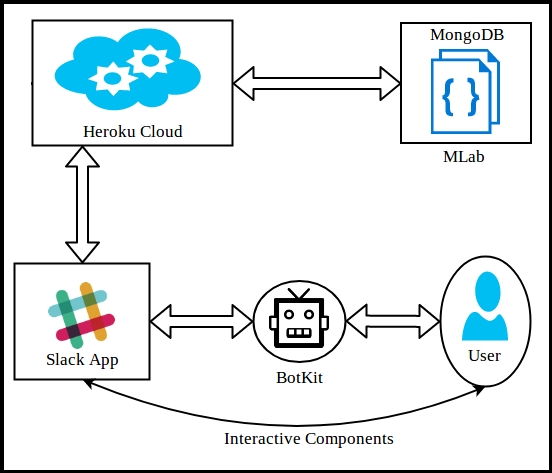
\includegraphics[height=0.5\textheight]{new_architecture.png}
\end{figure*}

Figure \ref{arch-pic} outlines the architecture of the application.
There are three main divisions: The user interface, the application server, and the database. 
Slack was used as the user interface. A custom bot was installed to that Slack page to handle 
interactive elements with the users. The applicaton was built with NodeJS. MongoDB was the 
database chosen to hold user data. For development purposes, a local server of NodeJS was run 
along with a local mongoDB database. Ngrok was used to tunnel webhooks between our local servers, 
which was necessary to get past local NATs and firewalls securely. The specific infrastructures are discussed as followed.


\subsubsection{Slack}
\label{sec:slack}

Slack is primarily a business tool intended to help facilitate
communication and coordination between individuals and groups at organizations.
In practice, however, Slack has become a familiar name with many unintended audiences such
as online communities and even university courses such as this one because of it's 
availability and ease of use. Attracting users to a platform they're already familiary with
is generally easier and less costly than attracting attention to a brand new website.

Another reason for using the Slack platform is that it already supports the languages and keyboard layouts for English, 
Japanese, German, Spanish, and French. Their website also claims to be 
including more regions in the future. Because of this, using a platform like Slack 
is beneficial to smaller developers as they can spend less time building a unique website 
and pushing it out internationally and more time on the functionality of the product. 

\paragraph{Slack Bot}
As mentioned previously, the target for this chat bot is to run in the Slack
platform. The Slack bot handles the interactions between the user and the NodeJS applications. 
All responses given by the user would be posted to the application by the bot. 
Similarily, all prompts sent to the user from application would be posted to Slack by the bot.

While it is true that this bot has been deployed to Slack specifically, it was
developed using a popular API called Botkit, which actually has APIs for
multiple chat services such as Facebook Messenger or Discord as well as Slack.
Because of this, it is possible to port WolfTutor to these other platforms
without needing to entirely start over.

%%% Local Variables:
%%% mode: latex
%%% TeX-master: "../main"
%%% End:


\subsubsection{NodeJS}
\label{sec:nodejs}
NodeJS is the primary framework being used in this project.  Node is a runtime
for Javascript which has proven to be strong competition for more traditional
LAMP stacks in the web.  In this case, it provides a number of different
libraries which make development of a chatbot easier.  Running Javascript also
has the benefit of making the chat bot easier to work on for a large number of
people given Javascripts ubiquity in recent years.

% Main.js file
\paragraph{Main.js}
Any interaction with the application via text is handled in the "main.js''
module. In this module are event listeners for text entry events in the Slack
chatbot.  Any time a student is typing a response or initiating contact with the
bot for the first time, the events for handling their inputs are in this file in
a series of listeners and callbacks.  Interestingly, the Botkit API used for
this project does not natively support a more modern JavasScript promise-based
design.

% Dialogs and Prompts
\paragraph{Dialogs and Prompts}
Dialogs are the other main way that students interact with the system.  In
Slack, a dialogue is a pop-up window that appears over the chat window and
contains web-controls such as text boxes, radio buttons, or drop-down select
boxes. These dialogs can be sent to the chat bot through the responses to user's
input in the ``main.js'' module, and can provide a richer interface for
providing structured data such as selecting subjects from a list or time slots
in a calendar.  The dialogs themselves also have a ``message response''
identifier which will be sent back to the slack bot when the user responds
which is the other primary way users interact with the system.  These response
identifiers provide an easy way to re-order or re-use messages without having to
make large code changes.  % TODO: justify that a bit?
Interestingly, slack only allows 5 controls to be in a single dialogue at one
time.  

% Modules
\paragraph{Modules}
The last major place for code is the modules folder.  The database access is
handled through the models but helpers are built around complex tasks and stored
in appropriate JS classes in the modules folder.  for example, the actual
database manipulation for tutors happens in the tutor model, but a tutor module
also exists that utilizes that module and adds business logic to it.  


%%% Local Variables:
%%% mode: latex
%%% TeX-master: "../main"
%%% End:


\subsubsection{MongoDB}
\label{sec:mongo}
MongoDB has serveral advantages. It is well documented for use with NodeJS, it is easy to set up a local database, it is also easy to set up online with MLAB platform and integrate into Heroku, and it is also easy to access through authorization credentials. Creating and uploading a mock database with a python script only took seconds with MLAB's authorization abilities to allow us to access the database outside of the MLAB site portal.


%%% Local Variables:
%%% mode: latex
%%% TeX-master: "../main"
%%% End:


\subsubsection{Heroku}
\label{sec:heroku}
Heroku is a popular cloud platform service that enables 
developers to run their applications online. Because of its 
popularity, there is an ample amount of documentation for using Heroku among other services such as NodeJS and mongoDB. Heroku also offers a free personal server that was used to speed up
in person evaluations of WolfTutor. To start the server, the single free dyno of the application's server would execute the Procfile via the 'npm start' command.


%%% Local Variables:
%%% mode: latex
%%% TeX-master: "../main"
%%% End:







%%% Local Variables:
%%% mode: latex
%%% TeX-master: "../main"
%%% End:


%%% Local Variables:
%%% mode: latex
%%% TeX-master: "../main"
%%% End:



\section{Evaluation}
\label{sec:evaluation}


\subsection{Algorithmic Evaluation}
\label{sec:algor-eval}
As we implement the enhancement of wolfTutor during each sprint, 
a variety of tests were conducted to verify the functionality and performance. 
For example, 1) unit tests were generated after the implementation of some 
core part, like prioritize method, so that to make sure the functionality of the 
new feature. 2) We also conducted a full user case manually tests after each 
sprint, to verify the functionality of the whole application. This means we fire 
up the server, mock the process by enrolling in the system,  becoming a tutor, 
switching to another user account, finding a tutor,  reviewing a previous tutor 
session, and also loading the history of previous tutor sessions.

In order to verify tutor matching algorithm quantitively, we define tutor 
suggestion accuracy as the percentage of how many the suggested tutors 
are in the good tutor set. The good tutor set was generated manually or 
automatically from a serial of matched tutors for a certain user, and this list 
of tutors will be considered as labeled good tutors. Then we ran our matching 
algorithm, logged the output and result into json files. Finally, we compared the 
output with the labeled good tutors and computed the accuracy.

\paragraph{Generate Dataset}
We need a database which contains a fair mont of user and tutor to work with. 
Manually adding users and tutors through the slack app interface will be too time-consuming. 
Instead, we designed and coded a script file in python. This script can automatically generate fix number of user and tutor, along with their random assigned attributes. For example, the user name and user email. But the most important attributes are the ones related to tutor experience and academic performance. These attributes are directly used in the matching and suggestion algorithms. This script can also impute those generated data into Mongo database, to provide test data during the user test and survey.

In this quantitative verification, we used this script to generated 300 users and 300 tutors. Each tutor was assigned a random number of reviews with random rating ranged from 1- 5. Each tutor also was assigned a random academic performance - GPA with a number ranged from 1-5. 

\paragraph{Test Design and Excution} 
test

\paragraph{Accuracy Result} 
test

%%% Local Variables:
%%% mode: latex
%%% TeX-master: "../main"
%%% End:


\subsection{Post Survey}
\label{sec:post-survey}


%%% Local Variables:
%%% mode: latex
%%% TeX-master: "../main"
%%% End:


\section{Responding to Change}
\label{sec:responding-change}
% TODO: Talk about the changes we made after the first round of tutori
The team performed evaluations in person and over two days.  At the end of
the first day, there were a few issues that had been consistently pointed out
that were fairly straightforward to fix.  To help focus on evaluating the speed
of use of the system, the team opted to fix a few of these issues immediately
before the second round of tutoring. 

\begin{figure}
  \caption{The tutor display prompt for a volunteer.} \label{fig:tutor_display}
  \centering
    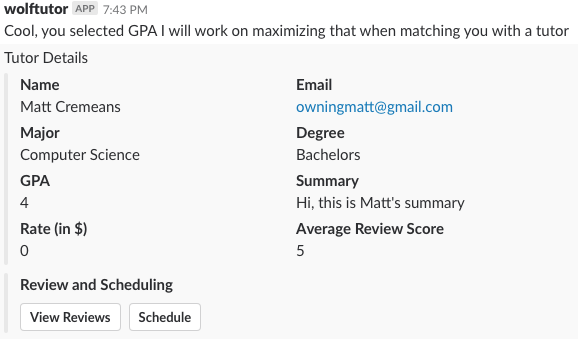
\includegraphics[width=0.5\textwidth]{tutor-display.png}
\end{figure}

% Fixed prompt to display rate as a currency
The first thing that was changed was a menu from the original system.  In the
original system, the tutor display had a ``Rate'' section that was intended to
display that tutor's billing rate.  During our trials, testers consistently
mistook this for a rating, so the team made the decision to add the quantifier
added in figure \ref{fig:tutor_display} switch things out.

% Added average tutor score to tutor display
The team also decided to add one other menu item. During the initial
development, the team intended to add average tutor review score to the same
tutor display discussed above, but overlooked that simple enhancement at the
time.  This made it more difficult for students to actually run the tests,
though it was still possible through the use of the original ``review'' view.
This field is also visible in figure \ref{fig:tutor_display}.

% Fixed order of tutors display
The final major change made after the first round of tutoring was a bugfix.
During the first round of evaluations, the team realized that the tutors being
displayed were displaying out of order from what the team expected.  After
investigating, it was discovered that the suggestion algorithm was not
malfunctioning as originally thought, but that the Slack API used to send the
tutor suggestions to the users was delivering messages asynchronously, rather
than synchronously as had been thought during development and initial testing.
This was rectified by changing to a different interface that, while slower
because it performed a handshake with every message, delivered the messages in
the correct order.  

%%% Local Variables:
%%% mode: latex
%%% TeX-master: "../main"
%%% End:



\section{Conclusion}
\label{sec:conclusion}

\subsection{Results}
\label{sec:results}

\subsection{Future Work}
\label{sec:future-work}
\subsubsection{Further Evaluation}
\label{sec:further-evaluation}
The team has made a best effort to evaluate the algorithm presented in this
paper both using a manually-labeled data set and using in-person interviews with
potential users. That said, true evaluation of educational software must be done
in a classroom setting.  

% TODO: describe ideal study
A good way to evaluate the usefullness of this system would be to truly put it
in the hands of students over a period of time. Over the course of several
semesters, a different set of sections of one course should be evaluated.  For
this reason, it may make sense to use a popular core course to a given major,
such as Intro to Computer Science.  These sections could be grouped into 3
groups, one with no intervention, one where students are pushed to use the
university-sponsored tutoring facilities that exist today, and one where
students are given access to the same facilities but are also given access to
WolfTutor.  Interviews would need to be conducted after student tutoring
sessions throughout the semester asking the students for feedback about the
quality of their tutoring session specifically and features of the application
more broadly.  At the end of the semester(s), the grades of the different groups
could be compared to historical data for the course and some generalizations
could be made about the usefulness of the software.

It is important to note, however, that an improvement in grades may not be the
right measure of success for this system. While better grades would certainly be
ideal, simply higher rates of engagement between students and tutors would be
one reasonable measure of success. Also, reducing time spent scheduling tutoring
sessions between students in the traditional tutoring section and WolfTutor
students would also be a reasonable win for students.  
% TODO: another method of evaluation is asking students to rate their tutors and
% seeing if they are consistently rating their tutors highly or poorly.

\subsubsection{Future Enhancement}
% TODO: describe the process of implementing a new algorithm in this setting
\label{sec:future-enhancement}
The other primary direction for future work is in the application itself.  The
recommendation module has been developed in isolation from the rest of the code
base, so it could easily be plugged into another process with minimal effort.
Whatever module simply needs to implement a method that takes in a list of
tutors and most of the integration work should be quite minimal.  The weighted
average that has already been implemented in this paper can serve as a good
baseline for future evaluation of other methods of classifying tutors.  Other
algorithms that might be a good fit for this problem are clustering algorithms
or classification algorithms.

Clustering algorithms may be a good fit because they all amount to identifying
groupings of similar entries in the population provided.  This is not unlike
what we want to do when searching for a tutor, so it might be possible to
cluster students and suggest tutors that exist in the same clusters as students.  

It is also possible that simple classification algorithms like logistic
regression on the simple end and SVM on the more complex end could be used to
classify tutors as good or bad.  That said, performance is a major concern in a
real-time application such as a chatbot, and such heavy algorithms as clustering
and classification may be too complex to run reliably in a production
environment.  

Another direction for future work is identifying more dimensions on which to
match tutors.  Currently we are matching on three review-related scores and one
academic performance score (gpa).  This could easily be expanded by asking
tutors and students more questions about what they are looking for.  Does the
student prefer test-taking or projects?  Do they speak English natively or would
they prefer to use some other language?  The team intended to implement more
dimensions to match on during the project, but time constraints forced limiting
it to four.  Fortunately, though, the application can easily be extended and
adding more dimensions is a fairly easy future direction.

%%% Local Variables:
%%% mode: latex
%%% TeX-master: "../main"
%%% End:


\subsection{Final Thoughts}
\label{sec:final-thoughts}
The final thought to conisder is whether or not group-p's contribution to
WolfTutor is truly an improvement over the existing system. In most fields, the
combination of the algorithmic evaluation provided in section \ref{sec:evaluation}
and the use validation provided in \ref{sec:evaluation} would be sufficent to
argue that the system is an improvement, but the education field is one that has
higher stakes than most.  

Educational data miners have spent considerable ink discussing the various
pitfalls in identifying high and low performers algorithmically, and the problem
of tutor recommendation is something that could potentially also be problematic.
If a student is connected with a poor tutor or one that handles their position
of power poorly, the potential impact could be catastrophic.  This may help
explain why many universities (such as Marshall University) require students to
take the courses they tutor for and bar anyone with lower than a B in that
subject from tutoring on top of requiring an in-person interview.

So does WolfTutor do enough to guarantee that a tutor is good or that they will
work well with the students?  The evaluation that has been done so far points
that it will make a good-effort to make recommendations that will ``do no harm''
but it would probably still make school administrators uneasy.  When combined
with a university vetting process, though, WolfTutor, especially after the
application of group-p's recommendations could serve universities and other
levels of schooling well as a platform for connecting students to peer tutors.  

%%% Local Variables:
%%% mode: latex
%%% TeX-master: "../main"
%%% End:


%%% Local Variables:
%%% mode: latex
%%% TeX-master: "../main"
%%% End:


\section{Chit}
\label{sec:chit}
\begin{itemize}
\item RHO
\item MEY
\item NOC
\item LJI
\item ZSO
\item CNM
\item YMA
\item YNH
\item VJK
\item PBZ
\end{itemize}

% REMOVE NOCITE OR IT WILL LIST EVERYTHING IN YOUR DATABASE AS A REFERENCE
% \nocite{*}

% Bibliography/style
\bibliographystyle{abbrv}

\bibliography{biblio}
% End bibliography/style

\end{document}
